\documentclass[runningheads]{llncs}
\AtBeginDocument{\pdfpagewidth=210mm \pdfpageheight=297mm}
\usepackage[T1]{fontenc}
\usepackage{lmodern}
\usepackage{graphicx}
\usepackage{amsmath,amssymb}
\graphicspath{{./}}
\begin{document}
\setcounter{section}{0}
\renewcommand{\thesection}{A}

\noindent\textbf{\large Preview --- Appendix A as it would appear in the paper}
\vspace{0.8em}\hrule\vspace{1em}

\section{From FIFO to the Recovered Front}
\label{app:beforeafter}

Figure~\ref{fig:beforeafter} makes the central allocation result legible at a
glance. The incumbent first-in, first-out (FIFO) policy and the 30-run combined
Pareto front are placed in the full three-objective space \emph{(a)} and then
read one objective at a time \emph{(b)}. FIFO is Pareto-dominated: it wastes
$1{,}940$ visas, whereas $94$ of the $104$ front solutions waste none; its
maximum inter-country disparity of $13.0$ years can be cut to $2.0$ years at a
cost of only ${\sim}2.4\,\%$ in the unserved waiting load $f_1$, on which FIFO is
already near-optimal and the front merely ties it. No single solution attains
all three extremes at once---that is precisely the trade-off the front
quantifies.

A striking corollary concerns how \emph{little} reallocation domination requires
(Figure~\ref{fig:country}). The $\min$-$f_1$ policy---the one that
Pareto-dominates FIFO---rescues $1{,}260$ of the incumbent's $1{,}940$ wasted
visas and puts them to use (reaching $139{,}320$ of the $140{,}000$ visas), and
it does so by changing only $2$ of the $21$ country totals; the remaining $19$
are unchanged and no objective is worse than FIFO. Equity-oriented points on the
front (e.g., the $\min$-$f_2$ extreme) redistribute far more---the structural
tension the front quantifies---so we display the dominating, minimal-disruption
policy here. All values are under the assumed synthetic model and constitute
auditable decision support; the totals illustrate method behavior, never a
recommended allocation.

\begin{figure}[t]
\centering
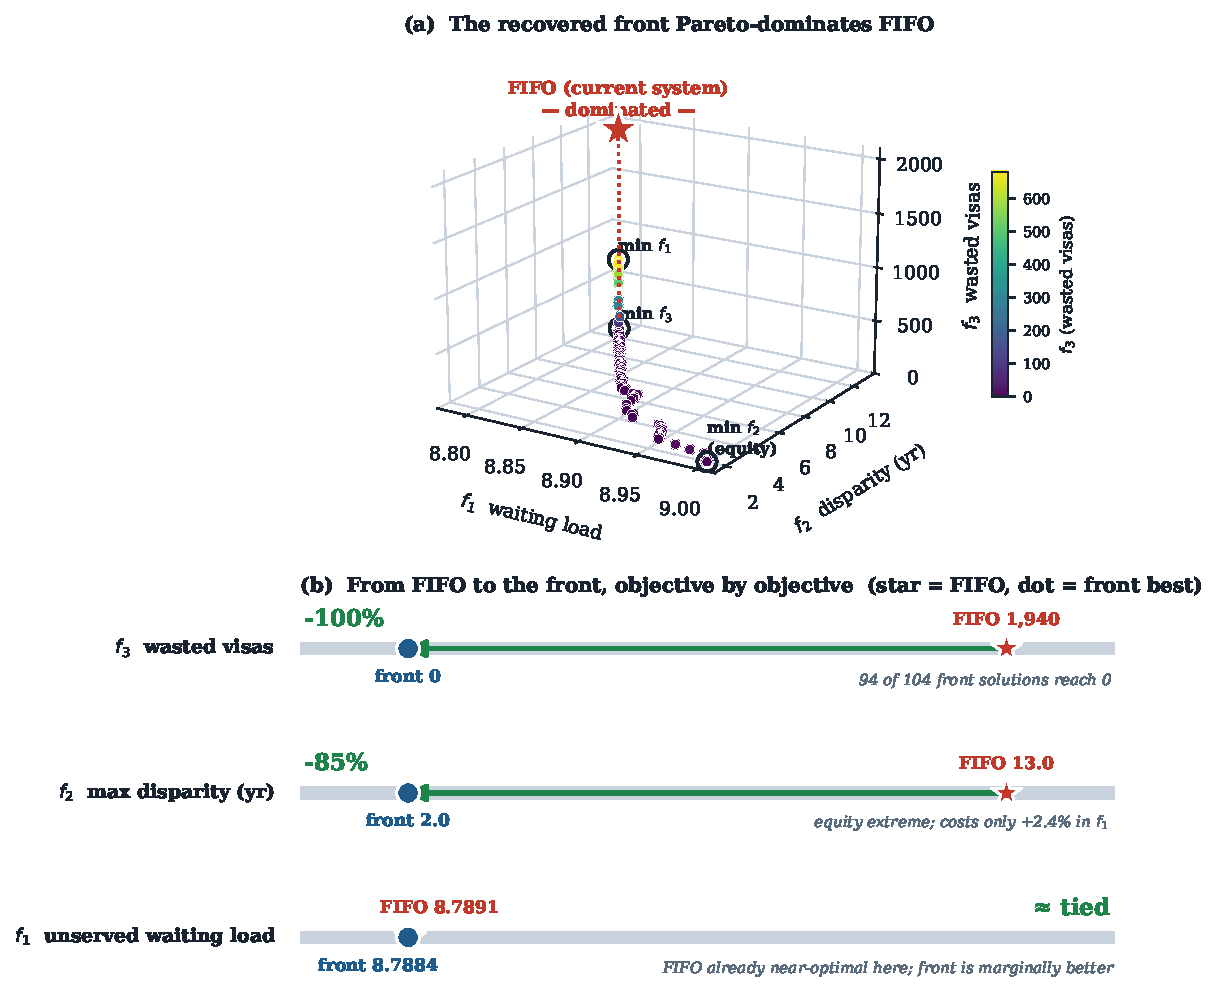
\includegraphics[width=0.93\textwidth]{fig_anexo_main.pdf}
\caption{From the FIFO incumbent to the recovered front (seeds 1--30).
\emph{(a)}~The 104-solution combined front in the full objective space, colored
by wasted visas $f_3$; the FIFO baseline (star) floats above the front and is
Pareto-dominated, with the three extreme solutions ringed. \emph{(b)}~The same
comparison objective by objective: wasted visas fall from $1{,}940$ to $0$
($94/104$ solutions), maximum disparity from $13.0$ to $2.0$ years (the equity
extreme, costing only $+2.4\,\%$ in $f_1$), while $f_1$ essentially ties FIFO
(the front is marginally better).}
\label{fig:beforeafter}
\end{figure}

\begin{figure}[t]
\centering
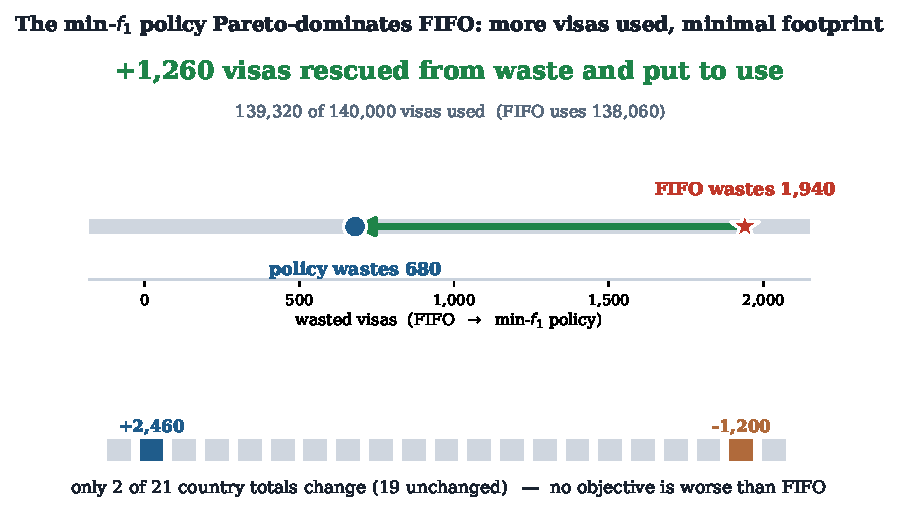
\includegraphics[width=0.92\textwidth]{fig_anexo_footprint.pdf}
\caption{How the $\min$-$f_1$ policy dominates FIFO (seeds 1--30,
firewall-verified front). It rescues $1{,}260$ of FIFO's $1{,}940$ wasted visas
(reaching $139{,}320$ of $140{,}000$ used) and changes only $2$ of the $21$
country totals, with no objective worse than FIFO. The totals illustrate method
behavior under the assumed synthetic model, not a recommended allocation.}
\label{fig:country}
\end{figure}

\end{document}
